% Chapter 1

\chapter{Methodology} % Chapter title

\label{ch:theory} % For referencing the chapter elsewhere, use \autoref{ch:introduction} 

%----------------------------------------------------------------------------------------

The project startup was officially set to be the 2nd of February with an expected turn-in date on the 10th of June. This time-span provided the group with approximately four months to complete the development of this project and the accompanying report.\\
The four months of official working time were divided into three overarching stages, in which we expected various parts of the project to have progressed a certain amount.\\ 

Here there will be a graph of how we used our time. \\

As far as the working schedule is concerned, we decided as a group on a fixed set of days each week, where the group would meet and work on the project. The rest of the days, each member of the group would work individually on pre-assigned tasks that would be discussed among the group in the next available meeting. Taking the above into account, we set a weekly schedule that was followed throughout the completion of this project (table XXX).\\

\begin{tabular}{ l | l | c | c | c | r | r }
Monday & Tuesday & Wednesday & Thursday & Friday & Saturday & Sunday \\
Meet & -- & -- & Meet & Meet & -- & Flex

\end{tabular} \\
\\

In an effort to maximize productivity and collaboration between group members, we decided to follow a classic software methodology, called SCRUM. This choice was made due to the fact that this project includes significant amount of programming work and most of the members have experience working under this method. \\
Being a sub-version of the Agile methodology, SCRUM adheres to a specific routine:

\begin{itemize}
\item Which tasks have been progressed since yesterday?
\item Which tasks will be worked on tomorrow?
\item Are there any obstacles preventing tasks from completion?
\end{itemize}

Always keeping in mind this routine, the three to four meetings scheduled each week were used to discuss the direction and progress of the project. 
During the meetings, group members could present propositions on how to enhance the project or seek assistance in the case where a task could not be completed. \\
In addition, other means of connection (Dropbox, Google Drive) were established in order to maintain communication among the group members on the days that group meetings did not occur. Furthermore, code was kept up-to-date between users, by using the code repository Github. This made it possible to all work on code at the same time, without diverging from the main script in general. \\
Developing the software and writing the report did not occur in parallel fashion, but extensive notes have been kept and a log was created in order to document the important issues and queries that occurred during the development phase. \\

The main issue that occurred during the development phase of the project was that in some cases, code needed to be tested on the server to determine whether it performed without any errors. That fact, crippled the flexibility of the group on the occasions where we needed to test fixes for broken code. To be more specific, each time a fix was implemented, the server needed to be restarted in order to load the new script and test its new version. When restarting the server we had to make sure that no other group member was working on the server side, so a waiting gap existed between fixing and testing the code.\\

\section{Previous Project}
As mentioned previously in this paper, this project is inspired by the work done during the second semester of our studies. In that project, we developed an ArcGIS toolbox which allowed the user to simulate a flood caused by the stowage of sea water. The aim of the project was to use ArcGIS geoprocessing modules to develop a user friendly model capable of modelling the mentioned phenomena. \\

\begin{figure}[h!]
\centering
	{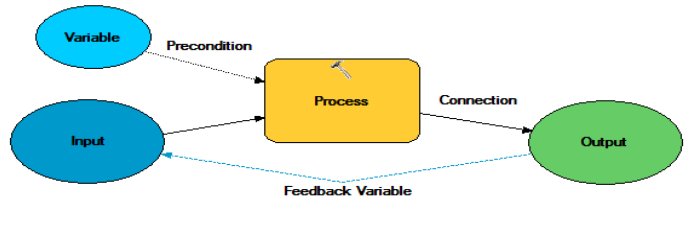
\includegraphics[width=\linewidth]{gfx/Methodology/old_project.png}}
\caption{The old model.}
\label{fig:inputs}
\end{figure}\\

The toolbox we created, comprised of ArcGIS functionalities with the core being the Cost Distance tool. The development was executed in with the built-in Model Builder. Model builder has the capability of invoking modules and algorithms through an easy-to-use Drag'N'Drop functionality. Although the preliminary model development is significantly easier due to the GUI, in order to apply more complex algorithm and connection between models models can quickly scale out of hand. 
The final tool made it possible to simulat water advancing through the landscape and covering parts of land that were below a certain predefined elevation, and were connected to the source of the flood. \\

After completing that project, we were left wondering how this toolbox could be made available to an even greater amount of people. Another question that arose was how this tool could be made available freely without any of the software limitations that using a proprietary licensed software, like the ArcGIS software suite, provide.
In order to pursue such an endeavor, we must make sure that this new product has to offer at least the same functionalities as the one created before. In addition, the way it is developed has to provide us with greater distribution potential in order to ensure widespread availability to any interested organization or person. Keeping these ideas in mind, we reached the aforementioned problem statement and begun working on this project.

\section{Workflow}
In order to be in accordance with the goals that we set, before working on the technical aspects of the project, we decided to split the project into several distinct phases. These phases comprise the general technical process we would have to go through when completing the project. They are created in such a way that they divide our work into parts that split our work into logical subparts. This division will also serve the purpose of making this report easier to read and more understandable to the reader.   
Based on this, we divided the project into a series of phases. Each phase describes a different process of the project from setting up its foundations to the final, fully working prototype. \\
The phases will be described as being distinctive from each other. In reality this is not the case. Since this is a product of group work, it made a lot sense to divide the workload among the different members of the group. This would save a significant amount of time since not all different phases required more than one member working on that specific part. That being said, the way the work unfolded, it resulted in overlapping phases. This simultaneous development of parts of the application ensured that constant communication among the group members was a high priority, this also made sure that changes on existing and fundamental parts were not too time consuming. For example, tweaking of the PyWPS  in order to connect and enable specific functions as they get developed to the server setup was a constant task throughout the entire project.\\

Below, is a quick sketch of how the phases were planned to look:

\begin{description}
	\item [Start-up:]
This phase involves defining exactly we wanted to attain with the project.

  \item[Phase 1:] In this phase we performed the core setup of the project. To be more specific, we decided on which server our data and functionalities will be deployed upon. In addition, we decided on the software and the programming languages  we will use. Finally, during this phase we setup the foundations we will base the work that will be performed in the following phases on.
  
  \item[Phase 2:] In this phase we deal with the conversion of the already created model to a model that is compatible with the choices we made on the phase before. In fact, this part does not deal with anything other than that conversion. It is the core of the process because the vital processes of the service are developed here.
  
  \item[Phase 3:] In this phase, we create the foundation of the web service. To be more specific, it involves the back-end of our service. How it is structured in order to support all the functionalities that will be provided to the user. 
  
  \item[Phase 4:] All the core functionalities of the applications are developed. This is the where the essence of the service is developed, from uploading an elevation model to creating a barrier and simulating the flood. 
  
  \item[Phase 5:]Here we mainly describe the front-end of the application. This is what the user sees and uses in order to get the results that he/she needs. It includes all interactive parts of the web service that initialize various functions  that provide the user with results.
  
  \item[Testing:] This is the final step of the implementation process. It involves experimenting with the various functionalities of the application and monitoring the way they affect the results. It also includes trying to predict how a user might try and use the software, and then seeing how that behavior will affect the process.
  
  \item[Writing:]As the project would become more and more finished, we will start the writing part. As mentioned we will keep notes, and write various parts that are important to memorize down as the project progresses, but the writing will occur mostly when the project is fully finished. This is done because some aspects of the project might change during the course of the development, and we don't want to have to redo various written parts, or we might even forget that they got changed, and forget to include the change in the project. 
  
  \item[Finishing up:]The final step is to make sure everything works, and to put a nice knot on the loose ends, as well as make sure that there is a red thread going through the project. Making sure that there is time to actually go through all the parts of the project is essential when doing a project such as this. 


\end{description}

The phases of the project will be explained in detail on the next chapter. The way we will present the development of our work is aiming in a more understandable and logically segmented report. That being said, we think that firstly presenting the final product that serves the purpose of its creation and then documenting the other unsuccessful routes that we tried is, for us, the best way to communicate our work to the reader. To be more specific, the layout of the next section of the report will provide the reader with the process of creating a working prototype in detail. This means that the various tools and techniques that we use will be presented and explained along with arguments on why we think that this is the best available solution at the time of creation. After we are finished with documenting this part, we spend some time presenting the alternatives that we tested before reaching to that solution, if there are any, and provide the reason and thoughts that lead us to abandon that specific course of action. By separating these two phases of development, we want to make sure that the reader can easily locate what they are looking for, i.e. suggested course of action or courses better avoided. 

\subsection{Founding the project in Denmark}

\subsection{Timeline}
We expected the various phases to take up approximately three weeks but with five weeks set aside for Phase 4 where the functions were developed, which would look something like \autoref{tab:phases}\\

\begin{table}
\centering
\begin{tabular}{l | c | c | r}
Phase & From & To & Duration \\

Start-up & 02/02/15 & 16/02/2015 & 14 \\
Phase 1 & 16/02/2015 & 09/03/2015 & 21 \\
Phase 2 & 02/03/2015 & 23/03/2015 & 21 \\
Phase 3 & 16/03/2015 & 06/04/2015 & 21 \\
Phase 4 & 30/03/2015 & 04/05/2015 & 35 \\
Phase 5 & 27/04/2015 & 18/05/2015 & 21 \\
Writing & 11/05/2015 & 03/06/2015 & 23 \\
Finishing up & 03/06/2015 & 10/03/2015 & 7
\end{tabular} \\
\caption{Phases and their allotted time}
\label{tab:phases}
\end{table}\\

Each phase has a weeks overlap with the previous phase. This is done to indicate that as one phase is slowly finishing up, the next one will slowly start up. This also shows how dynamic the creation of a project such as this is. \\
To give an overview of how we were expecting to progress with our project, we sketched the phases above into a so-called Gantt diagram. This gives a nice overview of this overlapping of the phases as mentioned above, and can be seen on \autoref{fig:gantt}.

\begin{figure}
\begin{ganttchart}[y unit title=0.4cm,
y unit chart=0.5cm,
vgrid,hgrid, 
title label anchor/.style={below=-1.6ex},
title left shift=.05,
title right shift=-.05,
title height=1,
bar/.style={fill=gray!50},
incomplete/.style={fill=white},
progress label text={},
bar height=0.7,
group right shift=0,
group top shift=.6,
group height=.3]{1}{20}
\gantttitle{Month}{20} \\
\gantttitle{February}{4} 
\gantttitle{March}{4} 
\gantttitle{April}{4} 
\gantttitle{May}{4} 
\gantttitle{June}{4}  \\

\ganttbar{Start-up}{1}{2} \\
\ganttbar{Phase 1}{3}{5} \\
\ganttbar{Phase 2}{5}{7} \\
\ganttbar{Phase 3}{7}{9} \\
\ganttbar{Phase 4}{9}{12} \\
\ganttbar{Phase 5}{12}{15} \\
\ganttbar{Writing}{15}{17} \\
\ganttbar{Finishing up}{17}{18} \\

\end{ganttchart}
\caption{Gantt-chart showing the overlap of phases}
\label{fig:gantt}
\end{figure}

%----------------------------------------------------------------------------------------
